%iffalse
\let\negmedspace\undefined
\let\negthickspace\undefined
\documentclass[journal,12pt,onecolumn]{IEEEtran}
\usepackage{cite}
\usepackage{amsmath,amssymb,amsfonts,amsthm}
\usepackage{algorithmic}
\usepackage{graphicx}
\usepackage{textcomp}
\usepackage{xcolor}
\usepackage{txfonts}
\usepackage{listings}
\usepackage{enumitem}
\usepackage{mathtools}
\usepackage{gensymb}
\usepackage{comment}
\usepackage[breaklinks=true]{hyperref}
\usepackage{tkz-euclide} 
\usepackage{listings}
\usepackage{gvv}                                        
%\def\inputGnumericTable{}                                 
\usepackage[latin1]{inputenc}                                
\usepackage{color}                                            
\usepackage{array}                                            
\usepackage{longtable}                                       
\usepackage{calc}                                             
\usepackage{multirow}                                         
\usepackage{hhline}                                           
\usepackage{ifthen}                                           
\usepackage{lscape}
\usepackage{tabularx}
\usepackage{array}
\usepackage{float}
\usepackage{multicol}
\usepackage{subcaption}

\newtheorem{theorem}{Theorem}[section]
\newtheorem{problem}{Problem}
\newtheorem{proposition}{Proposition}[section]
\newtheorem{lemma}{Lemma}[section]
\newtheorem{corollary}[theorem]{Corollary}
\newtheorem{example}{Example}[section]
\newtheorem{definition}[problem]{Definition}
\newcommand{\BEQA}{\begin{eqnarray}}
\newcommand{\EEQA}{\end{eqnarray}}
\newcommand{\define}{\stackrel{\triangle}{=}}
\theoremstyle{remark}
\newtheorem{rem}{Remark}


% Marks the beginning of the document
\begin{document}
\bibliographystyle{IEEEtran}
\vspace{3cm}

\title{NCERT-12.6.6.12}
\author{S. Sai Akshita - EE24BTECH11054}
\newpage
\maketitle
\bigskip

\renewcommand{\thefigure}{\theenumi}
\renewcommand{\thetable}{\theenumi}
\textbf{Question:} A point on the hypotenuse of a triangle is at distance $a$ and $b$ from the sides of the triangle. Show that the minimum length of the hypotenuse is $\brak{a^{\frac{2}{3}}+b^{\frac{2}{3}}}^{\frac{3}{2}}$.

\textbf{Theoretical Solution:}
Assume that $\theta$ be the angle between the hypotenuse and the height of the triangle, and $x$ and $y$ represent the portions of the hypotenuse corresponding to the lengths $a$ and $b$ projected along the hypotenuse.\\
The total length of the hypotenuse $c$ can then be written as:
\begin{align}
    c = x + y.\label{eq.1}
\end{align}
The relationships between $a$, $b$, $x$, $y$, and $\theta$ are:
\begin{align}
    x = a \sec\theta, \quad y = b \csc\theta.\label{eq.2}
\end{align}
Thus,by substituting \ref{eq.2} in \ref{eq.1}, the hypotenuse becomes:
\begin{align}
c = a \sec\theta + b \csc\theta.\label{eq.3}
\end{align}
To minimize $c$, we differentiate it with respect to $\theta$. Differentiating $c$ gives:
\begin{align}
\frac{dc}{d\theta} = a \sec\theta \tan\theta - b \csc\theta \cot\theta.\label{eq.4}
\end{align}
Setting $\frac{dc}{d\theta} = 0$ for critical points, we have:
\begin{align}
a \sec\theta \tan\theta = b \csc\theta \cot\theta.
\end{align}
Using trigonometric identities, this simplifies to:
\begin{align}
\frac{a \sin\theta}{\cos^2\theta} = \frac{b \cos\theta}{\sin^2\theta}.
\end{align}
Cross-multiplying:
\begin{align}
a \sin^3\theta = b \cos^3\theta.
\end{align}
Dividing through by $\cos^3\theta \sin^3\theta$ gives:
\begin{align}
\frac{\tan^3\theta}{1} = \frac{b}{a}.
\end{align}
Thus:
\begin{align}
\tan\theta = \brak{ \frac{b}{a} }^{\frac{1}{3}}. 
\end{align}
Using $\tan\theta = \left( \frac{b}{a} \right)^{\frac{1}{3}}$, we calculate $\sin\theta$ and $\cos\theta$ :
\begin{align}
\sin\theta = \frac{\tan\theta}{\sqrt{1 + \tan^2\theta}} = \frac{\brak{\frac{b}{a} }^{\frac{1}{3}}}{\sqrt{1 + \brak{ \frac{b}{a} }^{\frac{2}{3}}}},
\end{align}
\begin{align}
\cos\theta = \frac{1}{\sqrt{1 + \tan^2\theta}} = \frac{1}{\sqrt{1 + \brak{ \frac{b}{a} }^{\frac{2}{3}}}}.
\end{align}
Substituting these into \ref{eq.3}, we get:
\begin{align}
c = a \sqrt{1 + \brak{ \frac{b}{a} }^{\frac{2}{3}}} + b \sqrt{1 + \brak{ \frac{a}{b} }^{\frac{2}{3}}}.
\end{align}
Factoring and simplifying further, the result becomes:
\begin{align}
c = \brak{ a^{\frac{2}{3}} + b^{\frac{2}{3}} }^{\frac{3}{2}}.
\end{align}
Thus, the minimum length of the hypotenuse is:
\begin{align}
\boxed{c_{\text{min}} = \brak{ a^{\frac{2}{3}} + b^{\frac{2}{3}} }^{\frac{3}{2}}.}
\end{align}
\textbf{Gradient Descent Method for finding local minima:}\\ 
To find the value of $\theta$ for which the value of $c$ will be the lowest, Gradient Descent Method can be used iteratively. For that, we need to choose a random value for $\theta$, say $\theta_0$, and apply the method on repeat until we can be as close as we can to the local minima. The process is as follows:\\
We treat the length of the hypotenuse as a function of the angle $\theta$. \ref{eq.3}
\begin{align}
    c = a \sec\theta + b \csc\theta.
\end{align}
 By differentiating \ref{eq.3} and substituting the value of $\theta_0$, we get to know the slope of the tangent at that point. By moving along the downward side of tangent, and by using the following Iteration,
 \begin{align}
  \theta_{n+1} = \theta_n - \eta \times \frac{dc}{d\theta} \bigg|_{\theta = \theta_n}   
 \end{align}
By substitution, we get:
 \begin{align}
     \theta_{n+1} = \theta_n - \eta \brak{ \frac{a \sin\theta_n}{\cos^2\theta_n} - \frac{b \cos\theta_n}{\sin^2\theta_n} }
 \end{align}
Performing iterations,
\begin{align}
\theta_{1} &= \theta_0 - \eta \times  \brak{ \frac{a \sin\theta_0}{\cos^2\theta_0} - \frac{b \cos\theta_0}{\sin^2\theta_0} }\\
\theta_{2} &= \theta_1 - \eta \times  \brak{ \frac{a \sin\theta_1}{\cos^2\theta_1} - \frac{b \cos\theta_1}{\sin^2\theta_1} }\\
       \theta_{3} &= \theta_2 - \eta \times \brak{ \frac{a \sin\theta_2}{\cos^2\theta_2} - \frac{b \cos\theta_2}{\sin^2\theta_2} }
\end{align}
And so on ....\\
By opting certain value of $\epsilon$ such that 
\begin{align}
\left\lvert  \brak{ \frac{a \sin\theta_n}{\cos^2\theta_n} - \frac{b \cos\theta_n}{\sin^2\theta_n} } \right\rvert < \epsilon
\end{align}
We can obtain the minimizing value of $\theta$, i.e., $\theta^*$ such that $c\brak{\theta^*}$ is minimum. For this iteration, the smaller the values of $\eta$ and $\epsilon$ are, the greater the accuracy of the result will be.\\
\textbf{Theory vs Simulation plot assuming certain values:}
In order to plot theory vs sim plot, I'm assuming the values of $a$ and $b$ to be $2$ and $3$ respectively. Theoretically, the value of $\theta^*$ is $0.844$ radians. For simulation, I chose $\theta_0 = 0.1030$, $\epsilon = 0.000001$, and $\eta=0.0001$. This resulted in $\theta^*$ to be approximately $ 0.851$, which is almost the same value as the theoretical one. This shows the high efficiency of \textbf{Gradient Descent Method} in finding local minimas and maximas.

\begin{figure}[h]  
    \centering  
    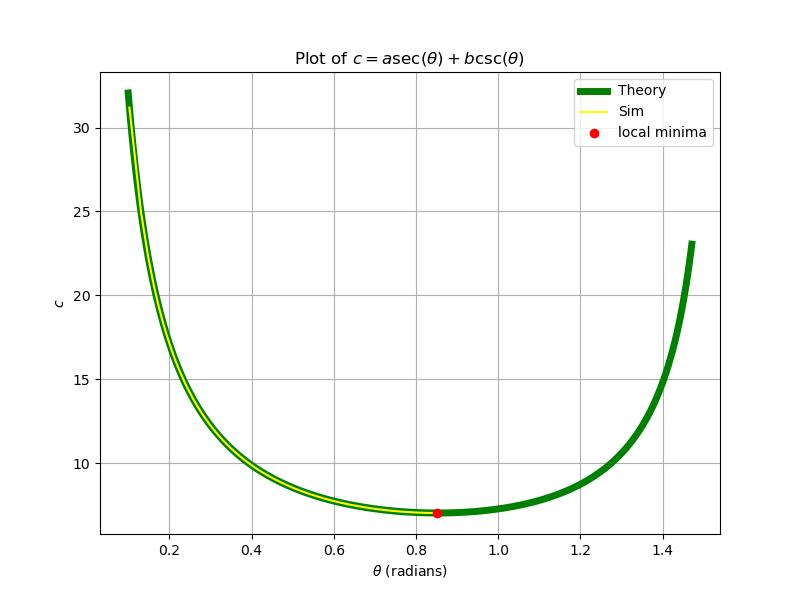
\includegraphics[width=0.8\linewidth]{Gradient.jpeg}   
    \label{fig:label}  
\end{figure}

 
\end{document}
